\chapter{Diseño}
\label{chap:design}

\section{Diseño de la interfaz gráfica}

\subsection{Pantalla principal}

\begin{figure}[ht]
	\centering
	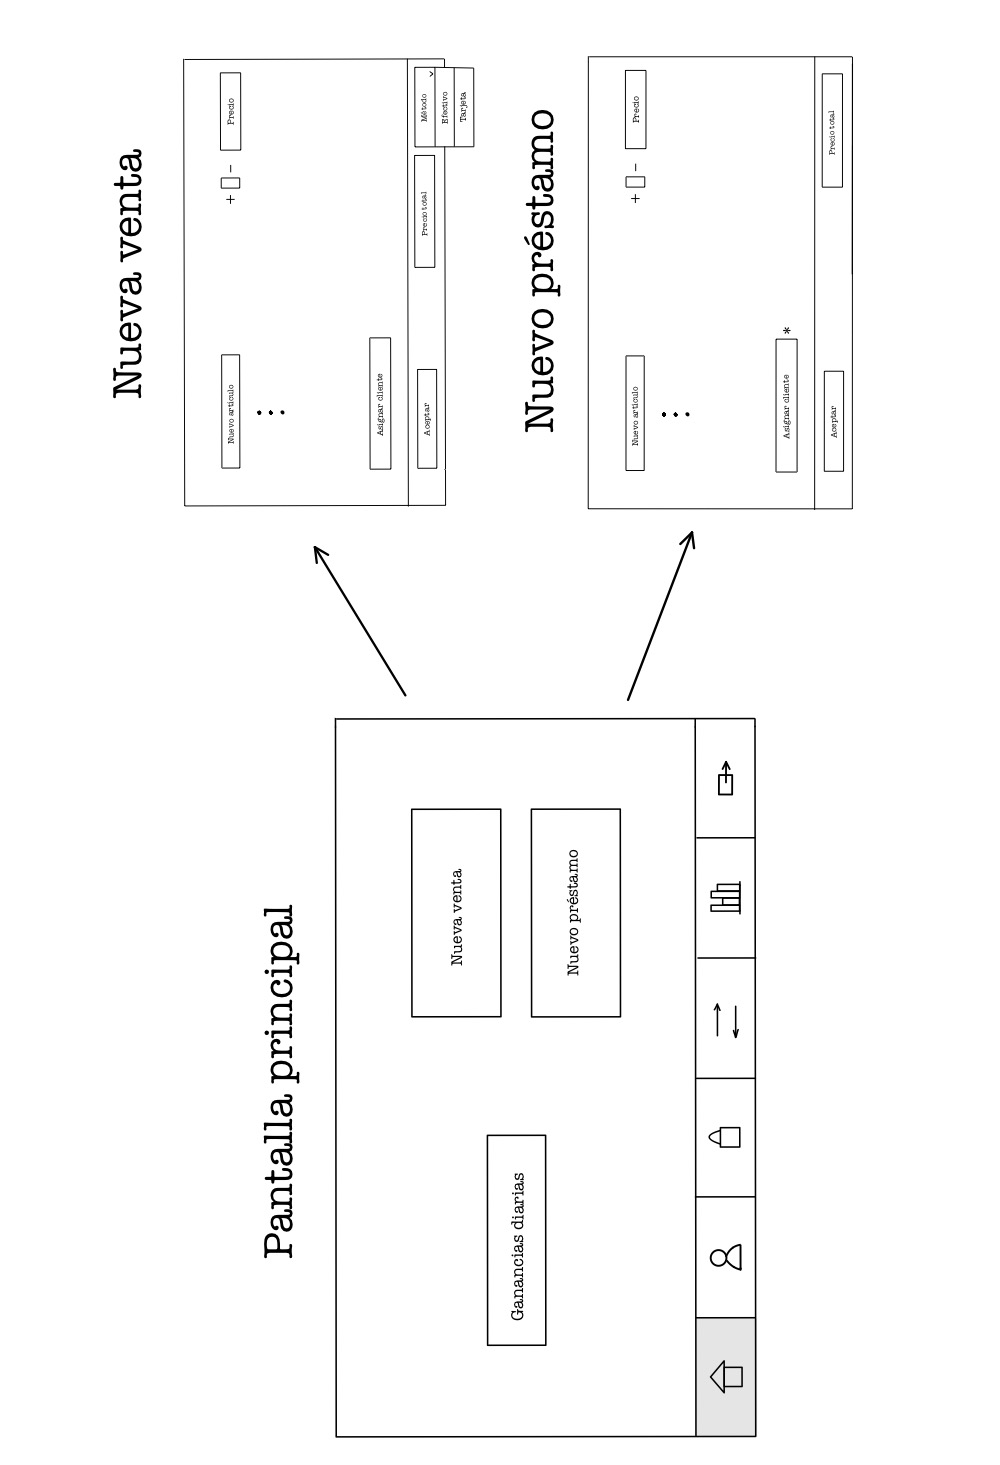
\includegraphics[width=0.8\textwidth, angle=270]{imagenes/pantalla_principal.JPG}
	\caption{Diseño de la pantalla principal.}
	\label{fig:pantallaprincipal}
\end{figure}



\subsection{Pantalla de clientes}

\begin{figure}[ht]
	\centering
	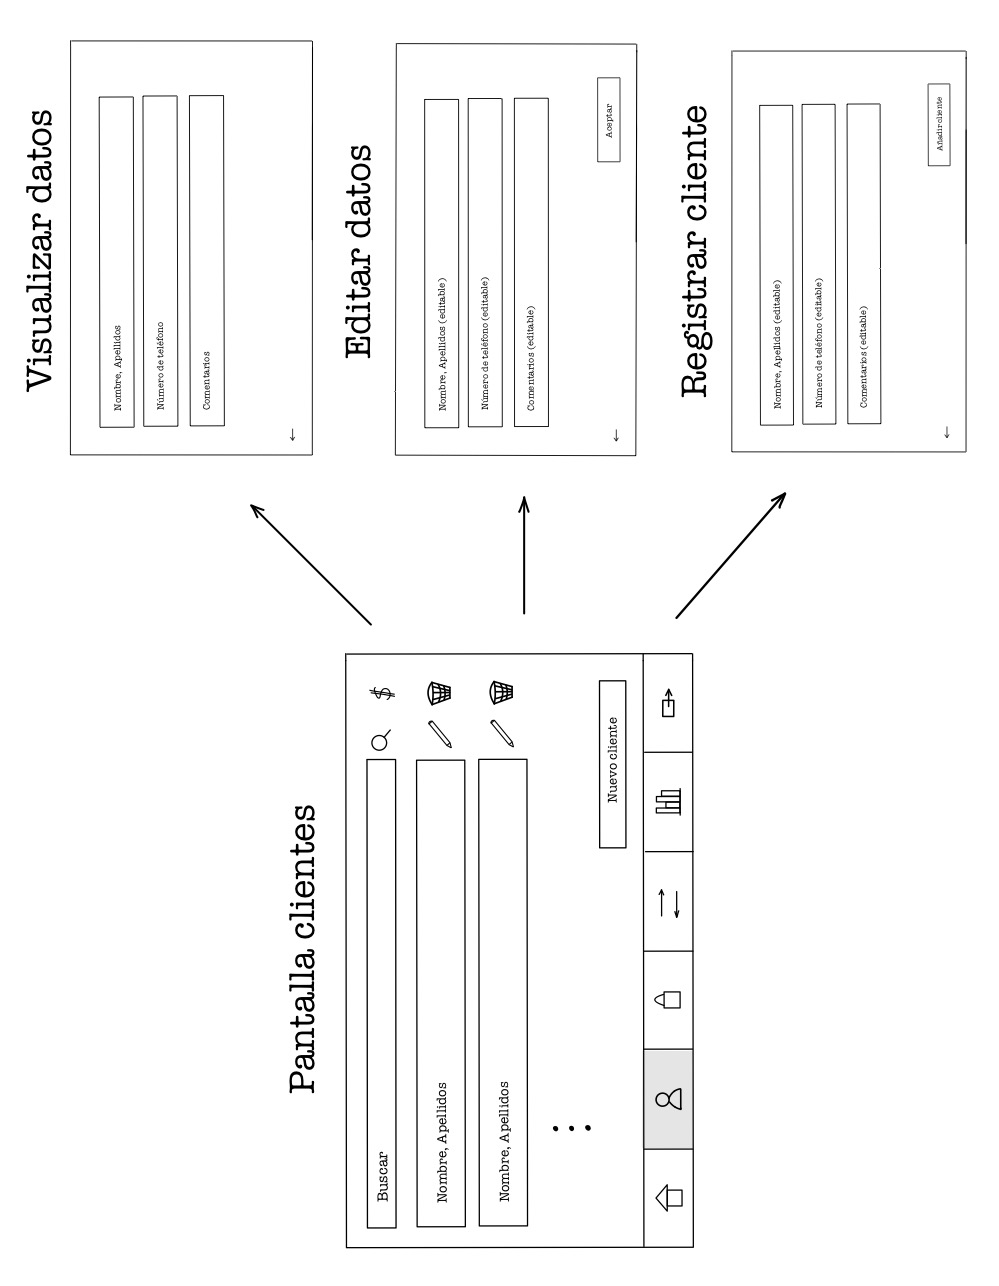
\includegraphics[width=0.8\textwidth, angle=270]{imagenes/pantalla_clientes.JPG}
	\caption{Diseño de la pantalla clientes.}
	\label{fig:pantallaclientes}
\end{figure}

\newpage

\subsection{Pantalla de artículos}

\begin{figure}[ht]
	\centering
	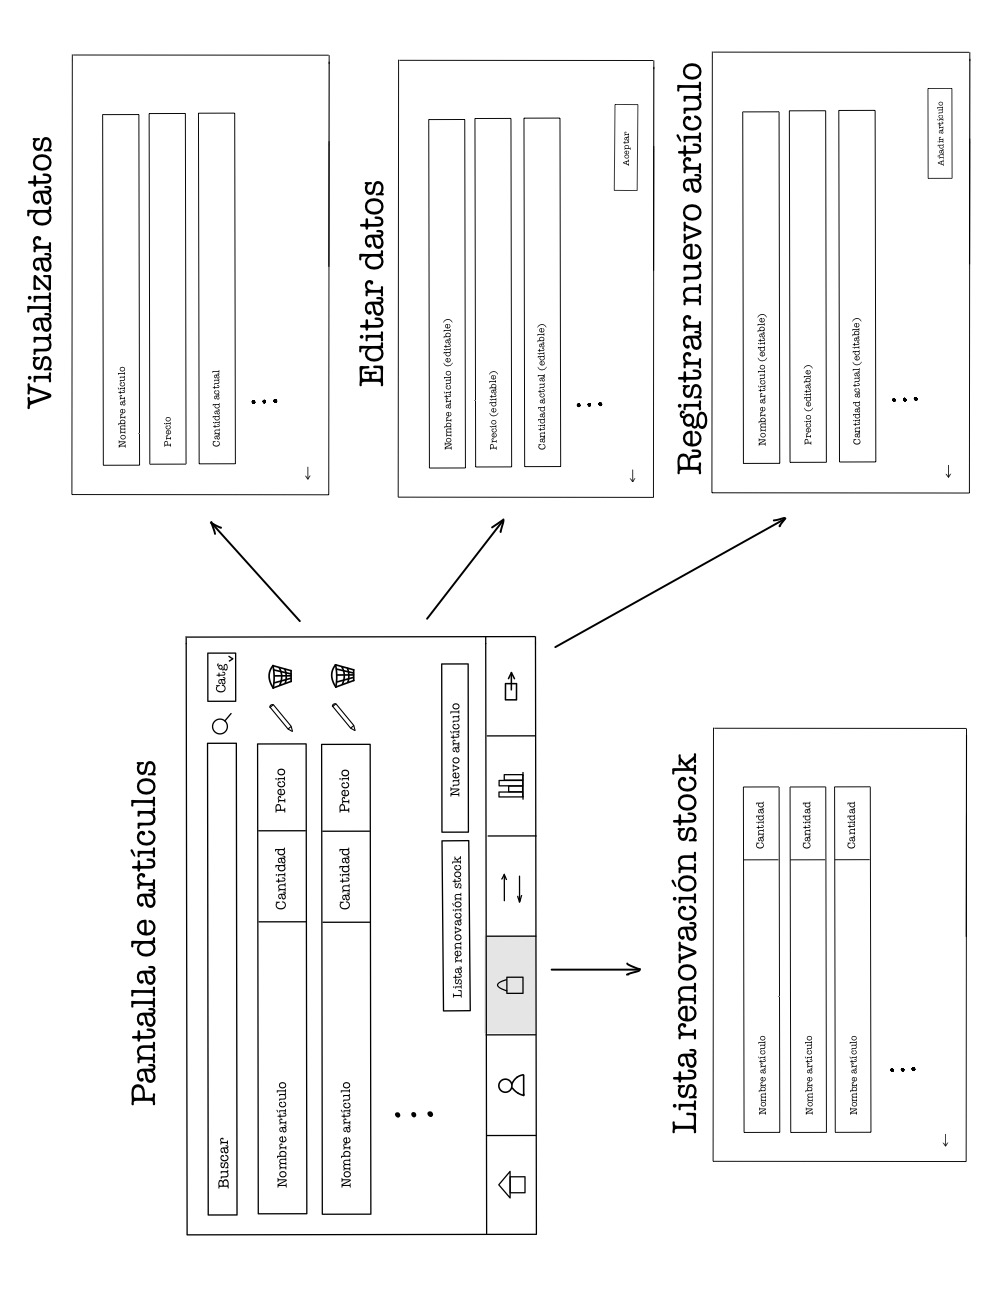
\includegraphics[width=0.8\textwidth, angle=270]{imagenes/pantalla_articulos.JPG}
	\caption{Diseño de la pantalla artículos.}
	\label{fig:pantallaarticulos}
\end{figure}

\newpage


\subsection{Pantalla de movimientos}

\begin{figure}[ht]
	\centering
	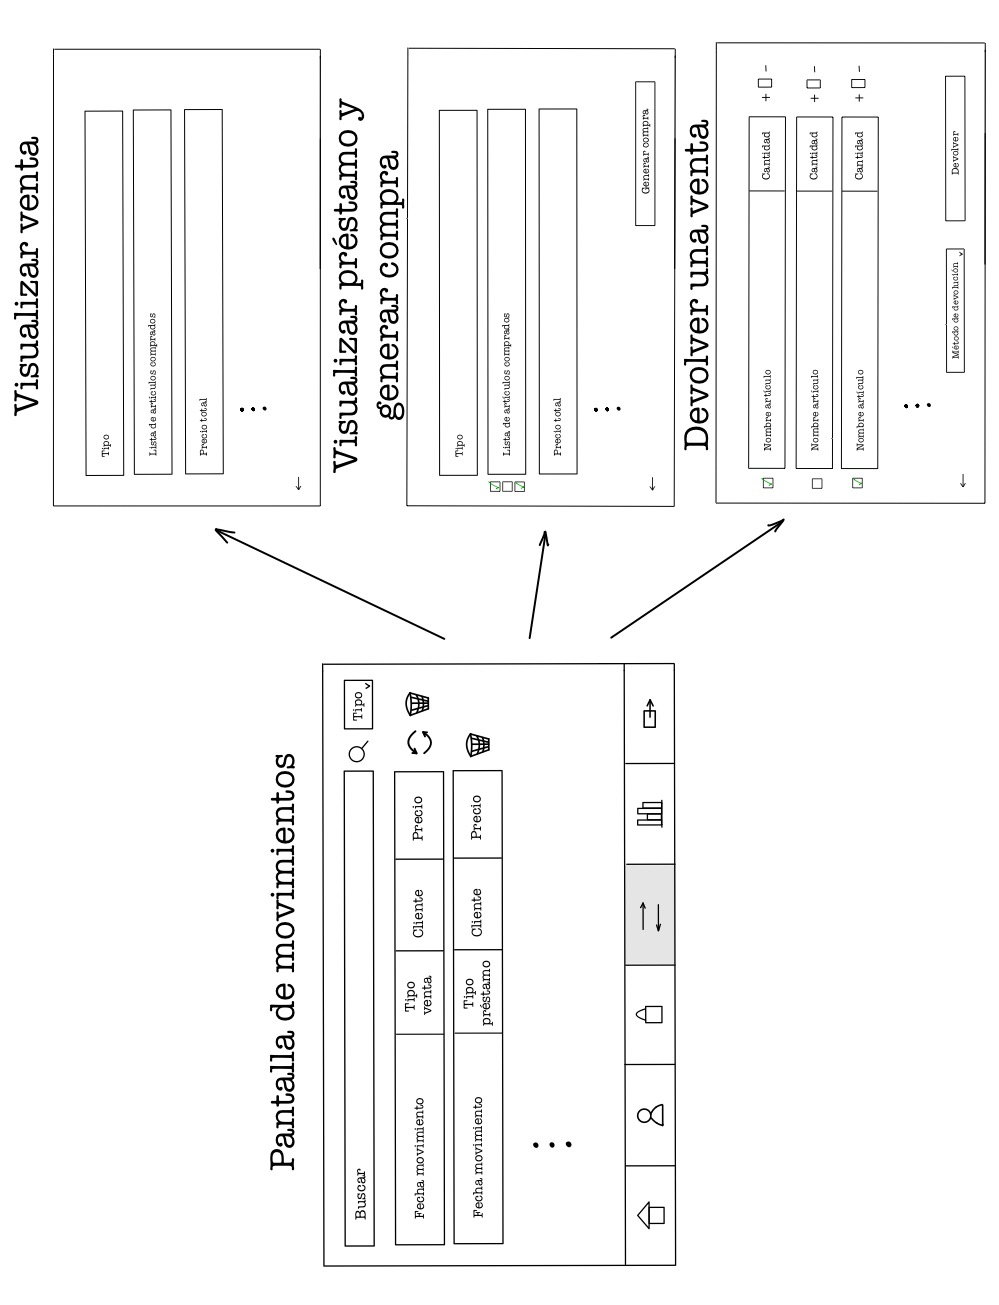
\includegraphics[width=0.8\textwidth, angle=270]{imagenes/pantalla_movimientos.JPG}
	\caption{Diseño de la pantalla movimientos.}
	\label{fig:pantallamovimientos}
\end{figure}

\newpage

\subsection{Pantalla de gráficos}

\begin{figure}[ht]
	\centering
	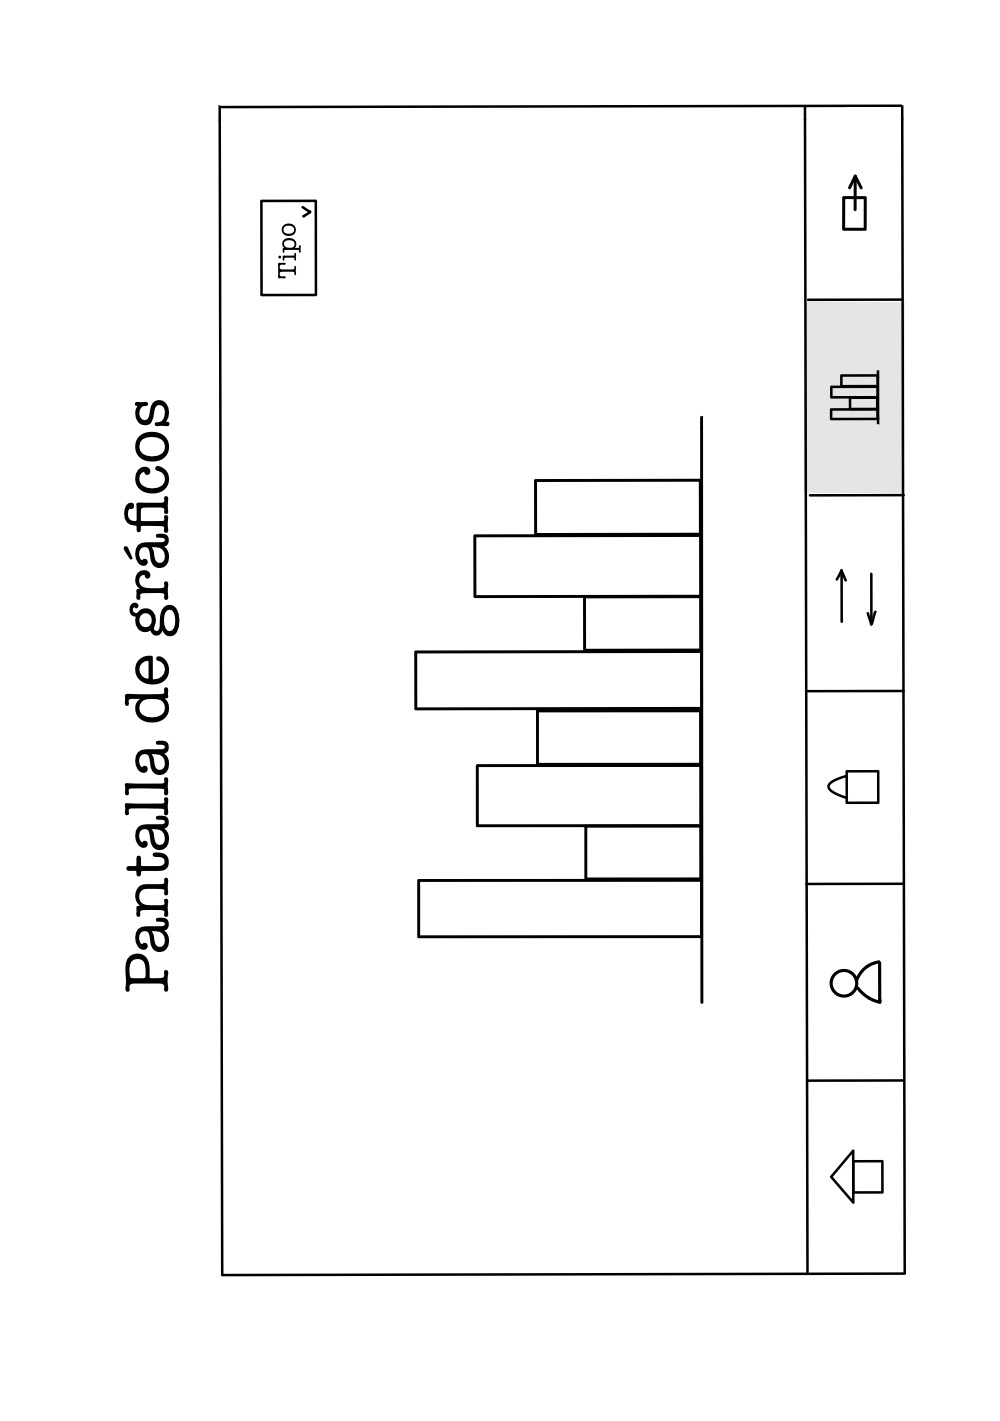
\includegraphics[width=0.8\textwidth, angle=270]{imagenes/pantalla_graficos.JPG}
	\caption{Diseño de la pantalla gráficos.}
	\label{fig:pantallagraficos}
\end{figure}